\documentclass[]{article}

\usepackage{amssymb}
\usepackage{amsmath}
\usepackage{geometry}
\usepackage{array}
\usepackage{multirow}
\usepackage{booktabs}
\bibliographystyle{apalike}

\usepackage{tikz}
\usetikzlibrary{shapes.misc}
\tikzset{cross/.style={cross out, draw=black, minimum size=2*(#1-\pgflinewidth), inner sep=0pt, outer sep=0pt}, cross/.default={2pt}} %default radius will be 2pt.

\begin{document}
\title{Specification}
\author{Erwan}
%\date{The 30th of January 2017}

\maketitle

\noindent Hereby we present the specifications for the constitution of a benchmark simulator thanks to which we will implement, test and compare funny algorithms in the context of Active Exploration of Unknown Environment for
Unmanned Aerial Vehicle.

\section*{Scenario}
We put ourselves in the context of the control of a glider drone flying in the open air. The environment has several characteristics namely:
\begin{itemize}
	\item it presents some convective atmospheric phenomenon allowing thermal soaring flight of the agent;
	\item it is uncertain -- the agent only knows a few things about its environment (detailed further);
	\item it is non-stationary -- the location of the thermals and more generally the wind field vary over time, increasing the uncertainty about the environment.
\end{itemize}
For the sake of illustration, a simplified 2D overview of the problem can be found in figure~\ref{fig:map}.

\begin{figure}[!h]
	\centering
	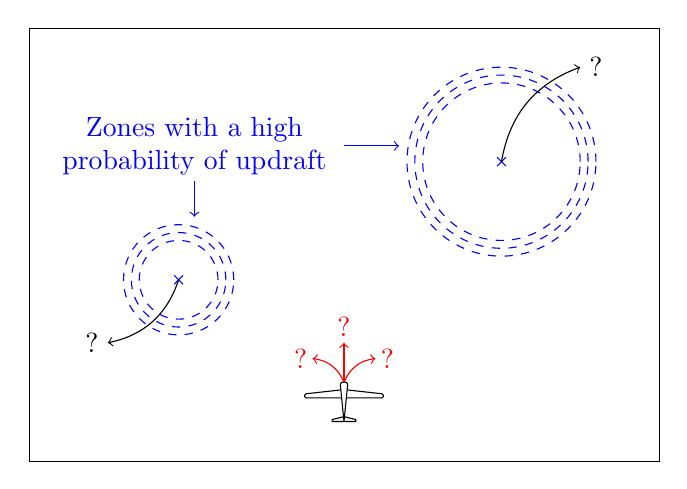
\begin{tikzpicture}[]
	% field
	\draw [ultra thin] (-4,-.5) rectangle (4,5);
	%\draw[step=0.5, gray, ultra thin] (-4,-.5) grid (4,5);
	
	% arrows
	\draw [->,red] (0,.5) -- (0,1);
	\draw [->,red] (0,.5) to[bend left] (.4,.8);
	\draw [->,red] (0,.5) to[bend right] (-.4,.8);
	\draw [red] (0,1.2) node {?};
	\draw [red] (.55,.8) node {?};
	\draw [red] (-.55,.8) node {?};
	
	% thermals 1
	\draw (-2.1,1.8) node[cross,blue] {};
	\draw [blue,dashed] (-2.1,1.8) circle [radius=.7];
	\draw [blue,dashed] (-2.1,1.8) circle [radius=.6];
	\draw [blue,dashed] (-2.1,1.8) circle [radius=.5];
	\draw [->] (-2.1,1.8) to[bend left] (-3,1);
	\draw (-3.2,1) node {?};
	% thermals 2
	\draw (2,3.3) node[cross,blue] {};
	\draw [blue,dashed] (2,3.3) circle [radius=1.2];
	\draw [blue,dashed] (2,3.3) circle [radius=1.1];
	\draw [blue,dashed] (2,3.3) circle [radius=1];
	\draw [->] (2,3.3) to[bend left] (3,4.5);
	\draw (3.2,4.5) node {?};
	% legend
	\draw [blue,text width=4cm, align=center] (-1.9,3.5) node {Zones with a high probability of updraft};
	\draw [->,blue] (-1.9,3.05) -- (-1.9,2.6);
	\draw [->,blue] (0,3.5) -- (.7,3.5);
	
	% big glider
	%\draw[thin,rounded corners=2pt] (0,0) -- (-.1,1) -- (.1,1) -- (0,0);
	%\draw[thin,rounded corners=1pt] (.1,.8) -- (1,.7) -- (1,.6) -- (.05,.6);
	%\draw[thin,rounded corners=1pt] (-.1,.8) -- (-1,.7) -- (-1,.6) -- (-.05,.6);
	%\draw[thin,rounded corners=0pt] (.01,.12) -- (.3,.05) -- (.3,0) -- (0,0);
	%\draw[thin,rounded corners=0pt] (-.01,.12) -- (-.3,.05) -- (-.3,0) -- (0,0);
	
	% small glider
	\draw[thin,rounded corners=1pt] (0,0) -- (-.05,.5) -- (.05,.5) -- (0,0);
	\draw[thin,rounded corners=.5pt] (.05,.4) -- (.5,.35) -- (.5,.3) -- (.025,.3);
	\draw[thin,rounded corners=.5pt] (-.05,.4) -- (-.5,.35) -- (-.5,.3) -- (-.025,.3);
	\draw[thin,rounded corners=0pt] (.005,.06) -- (.15,.025) -- (.15,0) -- (0,0);
	\draw[thin,rounded corners=0pt] (-.005,.06) -- (-.15,.025) -- (-.15,0) -- (0,0);
	\end{tikzpicture}
	\caption{Simplified 2D overview of the problem}
	\label{fig:map}
\end{figure}

%\noindent This environment has to be simulated within a software interfacing an environment model; an aircraft model; and a pilot. This environment model includes the model of the windfield that we rely on. Extensive study about thermal modeling has been done at ISAE (cf work with Srikanth) and can be considered here.

\noindent In this particular environment, we identified some missions that the agent has to fulfill. Table~\ref{tab:missions} gives a non-exhaustive list of the considered tasks. Each time we provided a short description of the mission and tried to identify the main difficulties.
Additionally, some extension to a motorized glider or any other aircraft like the very widespread quadcopter could be considered, as well as changes of the environment with the inclusion of obstacles for instance.
Indeed, the algorithms to be tested aim at wider applications that we would like to try in the future.
For now, we only consider the Thermal Soaring A and B missions.

\begin{figure}[!h]
	\centering
	\begin{tabular}{ m{2cm} m{.7cm} m{5cm} m{5cm} }
	\toprule
	Name & Label & Description & Difficulties \\ \midrule \midrule
	
	\multirow{2}{2cm}{Thermal Soaring} & A & The glider has to maximize its autonomy (altitude + velocity) in a convective situation i.e. inside a thermal. The latter is non-stationary, it can move and fade away. & Find the optimal trajectory maximizing the autonomy gain \\ \cmidrule(r){2-4}
	& B & The glider has to maximize its autonomy in a field of thermals whose positions are unknown. & Exploration-Exploitation trade-off within the updraft map \\ \midrule
	
	\multirow{2}{2cm}{Thermal Soaring + Travel} & C & The glider starts from a point A and has to go to a point B which is far away. In order to achieve this goal it needs to gain autonomy with Thermal Soaring.& Exploration-Exploitation trade-off within the updraft map + deal with potentially antagonist missions \\ \cmidrule(r){2-4}
	& D & Same as mission-C but with a list of points (A, B, C, ...). The list can be either ordered or not, meaning that the agent has to find its own path optimally. & Difficulties like in mission-C + establishment of a traveling plan \\ \midrule
	
	Thermal Soaring + Exploration & E & The glider has to fly by every places of a zone e.g. exploration mission. Obviously is must gain autonomy for the goal to be reachable. & Exploration-Exploitation trade-off within the updraft map + finding a shortest path trajectory for the exploration of the zone + deal with potentially antagonist missions \\ \midrule
	
	Thermal Soaring + Surveillance & F & The glider has to keep a zone under surveillance. An external player tries to reach a goal within this zone. & Have an optimal policy in the context of a 2-player game with a disequilibrium in the information access (the drone does not know the opponent's position and movement but the opposite is false)\\ \bottomrule
	\end{tabular}
	\caption{Table of the considered missions}
	\label{tab:missions}
\end{figure}

%\begin{figure}[!h]
%	\centering
%	\begin{tabular}{|m{3cm}|m{.85cm}|m{4.7cm}|m{4.7cm}|}
%		\hline
%		Name \T\B & Label & Description \T\B & Difficulties \T\B \\\hline\hline
%		
%		\multirow{2}{3cm}{\rotatebox{90}{Thermal Soaring}} & A & & cell3 \\\cline{2-4}
%		& B & cell6 & cello \\\hline
%		
%		Thermal Soaring & & \T The glider has to maximize its altitude i.e. autonomy \B & \T Exploration-Exploitation trade-off within the updraft map \B \\\hline
%		
%		Thermal Soaring + A-B Travel & & The glider has to gain enough autonomy in order to travel from a point A to a point B & \T Exploration-Exploitation trade-off within the updraft map + deal with potentially antagonist missions \B \\\hline
%		
%		Thermal Soaring + Exploration & & The glider has to gain enough autonomy in order to cover a zone to explore & \T Exploration-Exploitation trade-off within the updraft map + finding a shortest path trajectory for the exploration of the zone + deal with potentially antagonist missions \\
%		\hline
%	\end{tabular}
%	\caption{Table of the considered missions}
%	\label{tab:missions}
%\end{figure}

\section*{Simulator}

A Reinforcement Learning (RL) problem can be modeled as an agent-environment interface. As described in figure~\ref{fig:archi}, the environment is composed with an atmospheric model and an aircraft model together providing the agent with a next state $s'$ and a reward $r$ given an action $a$. Additionally, one can separate the absolute state space (state of the whole system) from the observable state space (available for the agent), dividing the notion of state space in two parts. In this section, we detail these seven components.\\

\begin{figure}[!h]
	\centering
	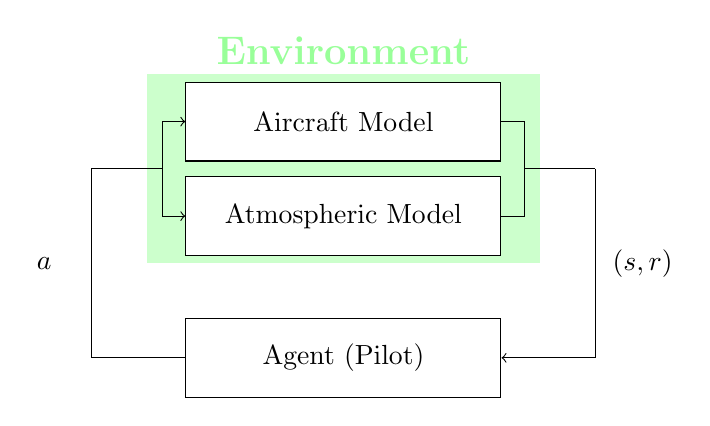
\begin{tikzpicture}[]
	% green box
	\draw [green!40!white,font=\bfseries] (0,1.5) node {\Large Environment};
	\fill [fill=green!20!white] (-2.5,-1.2) rectangle (2.5,1.2);
	
	% other boxes
	\begin{scope}[nodes={draw,fill=white,minimum width=4cm, minimum height=1cm, align=center}]
	\filldraw (0,+.6) node (airc) {Aircraft Model};
	\filldraw (0,-.6) node (envt) {Atmospheric Model};
	\filldraw (0,-2.4) node (pilt) {Agent (Pilot)};
	\end{scope}
	
	% nodes
	\coordinate (rcoord) at (+2.3,0);
	\coordinate (rrcoord) at (+3.2,0);
	\coordinate (lcoord) at (-2.3,0);
	\coordinate (llcoord) at (-3.2,0);
	\draw [->] (lcoord) |- (airc.west);
	\draw [->] (lcoord) |- (envt.west);
	\draw      (rcoord) |- (airc.east);
	\draw      (rcoord) |- (envt.east);
	\draw      (rcoord) -- (rrcoord);
	\draw      (lcoord) -- (llcoord);
	\draw [->] (rrcoord) |- (pilt.east);
	\draw      (llcoord) |- (pilt.west);
	
	\filldraw (+3.8,-1.2) node {$(s,r)$};
	\filldraw (-3.8,-1.2) node {$a$};
	\end{tikzpicture}
	\caption{Overall architecture}
	\label{fig:archi}
\end{figure}

\noindent \textbf{Atmospheric model;} we seek for a realistic model of the atmospheric phenomenon including the convective effects a.k.a. thermals. State of the art thermal models have been developed at ISAE based on the work of Allen. This model could be interfaced with any simulator and seems to be a good basis to start with. In addition, a global wind direction (constant wind field) and some noisy effects could be enough for our needs.\\

\noindent \textbf{Aircraft model;} we used a 1 point dynamic model of the aircraft in former work about the same subject \cite{beeler2003flight}. This simple model allows us to recreate realistic behavior of a glider drone and can be reused in a first time. However, some model instabilities have been spotted, particularly when it is about setting a maximum threshold in the range of the attitude angles. Thus, we can either decide to fix these issues in order to keep on working with it or chose another model. It could be interesting to use a benchmark model such that those provided by the open source flight simulator JSBSim. Indeed, the use made of the latter in the scientific community allows for more visibility.\\

\noindent \textbf{Absolute state space;} it includes the whole information about the state of the aircraft and the environment. Detailing a specific format is not necessary here and will depend on technical considerations relative to the code.\\

\noindent \textbf{Observable state space;} it includes what the agent sees i.e. the information harvested by the sensors. Here we try to establish an exhaustive list:
\begin{itemize}
	\item $(x,y,z)$ the position in the 3D space, practically acquired by a GPS system and in our case we can simply access its real value used for the environment's transition;
	
	\item $(V, V_{air}, V_{wind})$ respectively the velocity of the aircraft in the earth frame acquired with a GPS; the velocity of the wind in the aircraft frame acquired with a pitot tube; and the velocity of the wind in the earth frame which can be obtained via the following formula:
	\begin{equation*}
		V = V_{wind} - V_{air}
	\end{equation*}
	
	\item $(\theta, \phi, \psi)$ respectively pitch angle, roll angle and yaw angle, representing the attitude of the aircraft in the earth frame;
%	\begin{figure}[!h]
%		\centering
%		\begin{tikzpicture}[]
%			% earth frame
%			\draw[thick,->] (0,0,0) -- (5,0,0) node[anchor=west]{$east$};
%			\draw[thick,->] (0,0,0) -- (0,5,0) node[anchor=west]{$vertical$};
%			\draw[thick,->] (0,0,0) -- (0,0,-5) node[anchor=west]{$north$};
%		\end{tikzpicture}
%		\caption{Attitude of the aircraft}
%		\label{fig:pitchrollyaw}
%	\end{figure}
%	\begin{figure}[!h]
%		\centering
%		\includegraphics[width=6cm]{img/roll_pitch_yaw.jpg}
%	\end{figure}

	\item $(\alpha,\beta)$ respectively angle of attack and side slip angle, the first represents the angle between the direction of the airflow and the aircraft's reference line (e.g. chord line), the second is the angle between the velocity vector and the aircraft plane of symmetry;
	
	\item $(\gamma, \chi)$ respectively the flight path angle representing the angle between $V$ and the earth horizontal; and the course heading representing the angle between $V$ and the vector indicating the north in the earth frame. We have the following formula:
	\begin{align*}
		\gamma &= \theta - \alpha \\
		\chi &= \psi + \beta
	\end{align*}
	
	\item the rate of the aforementioned quantities, especially the climbing rate $\dot{z}$ measuring the vertical velocity of the aircraft in the earth frame;
	
	\item Vision-based data: here is a tricky one, we intend to use vision based data giving some clue about the position of the thermals (clouds for instance). The difficulty is that it has to be uncertain in a realistic way. Some clouds indicate the presence of a thermal but some thermals do not have clouds and vice versa. We propose to simulate the effect by randomly decide on the presence of a cloud on top of a thermal. Additionally some clouds can be randomly added to the environment. The input given to the glider could be the position of clouds in the vision field.
\end{itemize}

\noindent \textbf{Reward;} the reward is essentially built with the data of the absolute state space accordingly to the chosen mission.\\

\noindent \textbf{Action space;} several level of actions can be defined, from the lower to the higher we can have the following: the actuators control; the attitude of the aircraft described in the state space; and the trajectory of the aircraft. From a spatial point of view i.e. if we characterize the environment spatially (for instance if there is a cloud at position $(x_c,y_c)$ how can I get there) it can be convenient to consider the action space as a trajectory space. However more practically with respect to what we control on board of a UAV the attitude of the aircraft seems more realistic.\\

\noindent \textbf{Agent;} The agent is the pilot i.e. the policy realizing the processing of the harvested data and the deterministic or probabilistic mapping between state and action. No definition is provided here.\\

\noindent The aforementioned observable state space is fully detailed, but it is not relevant to consider its entirety for every missions. We separated the relevant features of the state space with respect to the missions presented in table~\ref{tab:missions} in table~\ref{tab:obsstates}. Similarly the action space is not always the same and details are also provided in this table.

\begin{figure}[!h]
	\centering
	\begin{tabular}{m{3cm} m{5cm} m{5cm} }
		\toprule
		Mission Label & Relevant state components & Relevant action components \\ \midrule \midrule
		
		A & $V_{earth}, \dot{z}$ & $\theta, \phi, \beta$ \\ \midrule
		
		B, C, D, E, F & $V_{earth}, \dot{z}, x, y, z, Vision$ & $\theta, \phi, \beta$ or $\dot{x}, \dot{y}, \dot{z}$ \\ \bottomrule
	\end{tabular}
	\caption{Table of the relevant state and action components for each mission presented in table~\ref{tab:missions}}
	\label{tab:obsstates}
\end{figure}

\bibliography{mybib}

\end{document}
